\begin{enumerate}
    \item[\textred{3.}(a)] Suppose you have two sequences, \{24, 19, 12, 6, 24, 36, 40, 39\} and \{6, 12, 24, 19, 39, 40, 36, 24\}. You know the first one is generated from some BST A by pre-order tree walk, and the second one is generated from some BST B by post-order tree work. Please draw all the possible BST A that can generate the sequence. Repeat that for BST B.
\begin{figure}[!h]
    \centering
    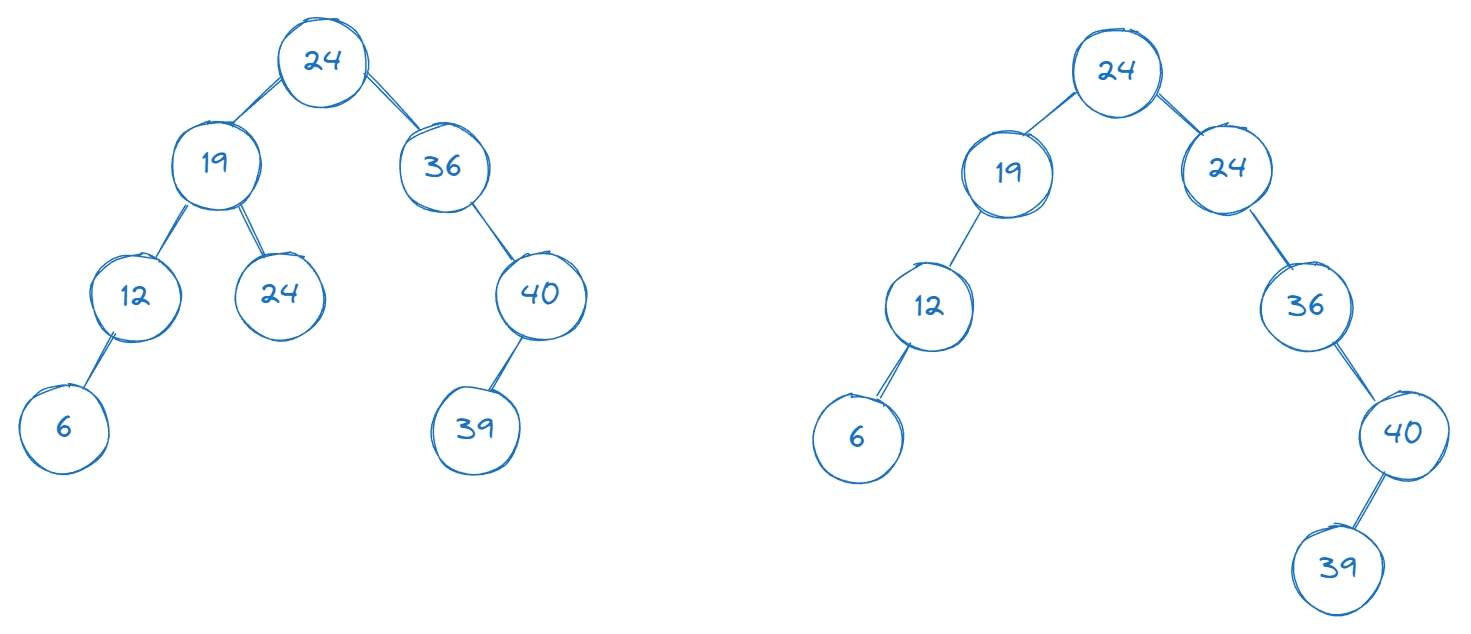
\includegraphics[width=0.9\linewidth]{HWs/HW6/figures/3-1.png}
    \caption{3.(a) Two possibilities of BST A}
    \label{fig:bst-a}
\end{figure}
\begin{figure}[!h]
    \centering
    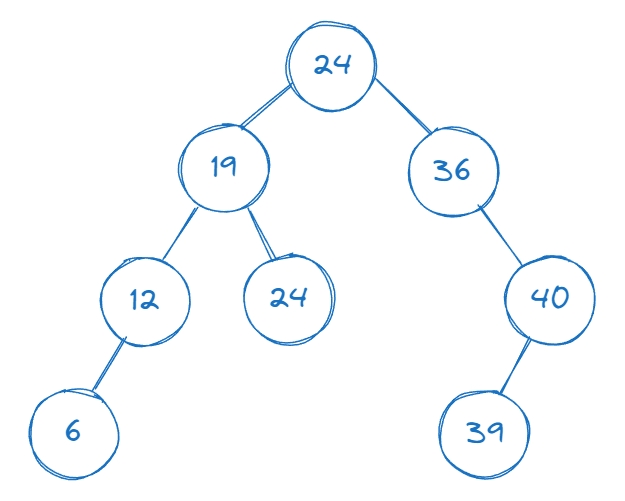
\includegraphics[width=0.4\linewidth]{HWs/HW6/figures/3-2.png}
    \caption{3.(b) The only possibility of BST B}
    \label{fig:bst-b}
\end{figure}
    \item[(b)] If all the keys in a BST are distinct, can you draw a unique BST when only given its pre-order tree walk? If yes, please describe why; if no, find a counter-case.\\
    \textblue{
    Yes. The first element in the pre-order traversal is always the root. And as we move through the pre-order traversal, we can compare each element with the previous element. If it is smaller, then it belongs to the left sub-tree; vice versa, it belongs to the right sub-tree of it's parent.
    }
\end{enumerate}
